\documentclass[superscriptaddress,prx, showkeys]{revtex4}
\usepackage{amssymb}
\usepackage{color}
\usepackage{xcolor}
\usepackage{amsmath, amsthm, amssymb,amscd, mathrsfs, amsfonts, mathtools}
\usepackage{tikz}
\usetikzlibrary{matrix,arrows,decorations.pathmorphing}
\usetikzlibrary{backgrounds}
\usetikzlibrary{shapes.geometric}
\usepackage{circuitikz}
\usepackage{tcolorbox}
\tikzset{1simpl/.style={->,>=stealth,thick}}
\tikzset{vertex/.style = {circle, draw, fill=red, inner sep=1}}

\begin{document}

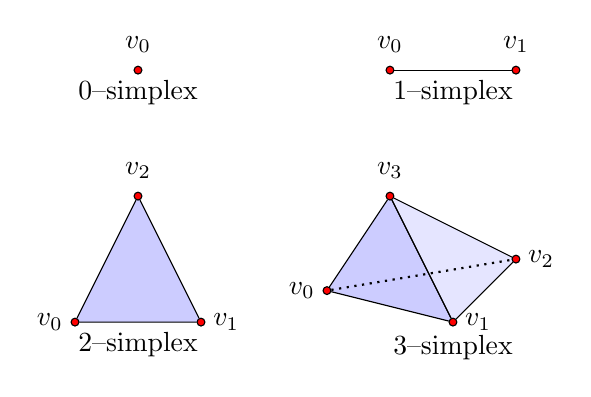
\begin{tikzpicture}[scale=.8]
  %% 0-simplex
  \node[vertex] (0) at (0,0) {};
  \node at (0,0.4) {$v_0$};
  \node [below] at (0,0) { 0--simplex};
  
  %% 1-simplex
  \node[vertex] (v00) at (4,0) {};
  \node[vertex] (v01) at (6,0) {};
  \node at (4,0.4) {$v_0$};
  \node at (6,0.4) {$v_1$};
  \draw[-] (v00) -- (v01) node[midway, below] { 1--simplex};
  
  %% 2-simplex 
  \node[vertex] (v0) at (-1,-4) {};
  \node at (-1.4, -4) {$v_0$};
  
  \node[vertex] (v1) at (1, -4) {};
  \node at (1.4, -4) {$v_1$};
  
  \node[vertex] (v2) at (0,-2) {};
  \node at (0, -1.6) {$v_2$};
  
  \draw[-] (v0) -- (v1) node[midway,below] { 2--simplex}  -- (v2) -- (v0);
  %% fill the triangle
  \begin{scope}[on background layer]
  \fill [blue!20] (v0.center) -- (v1.center) -- (v2.center) -- cycle;
  \end{scope}
  
  %% 3-simplex
  \node[vertex] (vv0) at (3, -3.5) {};
  \node at (2.6, -3.5) {$v_0$};
  
  \node[vertex] (vv1) at (5, -4) {};
  \node at (5.4, -4) {$v_1$};

  
  \node[vertex] (vv2) at (6, -3) {};
  \node at (6.4, -3) {$v_2$};
  
  \node[vertex] (vv3) at (4, -2) {};
  \node at (4, -1.6) {$v_3$};
  
  \draw (vv0) -- (vv1) -- (vv3) -- (vv0);
  \draw (vv1) -- (vv2) -- (vv3) -- (vv1);
  \draw[dotted, thick] (vv0) -- (vv2);
  
  
  \begin{scope}[on background layer]
  \fill[blue!20] (vv0.center) -- (vv1.center) -- (vv3.center) -- cycle;
  \fill[blue!10] (vv1.center) -- (vv2.center) -- (vv3.center) -- cycle;
  \end{scope}
  \node at (5, -4.4) { 3--simplex};
  
\end{tikzpicture}

\end{document}